\section{Microsoft Kinect}
En Kinect er et Natural User Interface (NUI) udviklet til Microsoft's spillekonsol, Xbox.
Den gør det muligt at interagerer med sin konsol ved at bevæge kroppen og via talte kommandoer.
Den første version der udkom i november 2010~\cite{kinectWiki} er oprindeligt udviklet med henblik på at lokke nye typer brugere til Xbox med det argument at det via naturlig (og aktiv) bevægelse er sjovere og mere virkelighedstro at spille.

Dog blev der i februar 2012 lanceret en ny type Kinect, kaldet Kinect for Windows, der sammen med et Software Development Kit (SDK), gør det muligt at udvikle både kommercielle og non-kommercielle applikationer til Kinect som også kan eksekveres på Windows platformen.
Kort fortalt er Microsoft's Kinect mere end en input enhed gamere kan bruge for at gøre deres spiloplevelse mere virkelighedstro; af andre anvendelser kan f.eks. nævnes~\cite[s.~17]{kinectProgrammingGuide}:

\begin{itemize}
\item Optagelse af video i real-tid
\item Generere et dybde billede ved hjælp af kameraet og de to IR sensorer
\item Sende talte kommandoer
\item Vurdering af omgivelserne ved hjælp af lyd
\end{itemize}

Dette er alle interessante eksempler der på hver deres måde kan afhjælpe problemet med at bestemme en autonom robots placering i ukendte omgivelser.
Derfor vil Kinecten, både med hensyn til hardware, men også til software blive nærmere beskrevet i de følgende afsnit.


\subsection{Opbygning af Kinect}
I denne rapport er det versionen Kinect for Windows der fokuseres på, da den giver bedst kompatibilitet med PC samt det faktum at den er tilgængelig gennem universitetet.

Dog kan det nævnes at forskellene mellem den og versionen til Xbox er meget små.
Hardware mæssigt har Kinect for Windows den fordel at firmwaren indeholder en såkaldt Near Mode, hvilket gør det muligt at følge objekter indtil 40 cm fra enheden.
Kinect for Xbox har ikke denne funktionalitet, og kan derfor kun følge objekter indtil 80 cm fra enheden, hvilket kan blive et problem i situationer hvor man ønsker at detektere små afstande via dybdebilleder.
Kinect for Windows kan desuden også benyttes til kommercielle applikationer, hvor dens pendant er beregnet til hobbyister, generel udvikling og forskning~\cite[s.~16]{kinectProgrammingGuide}.

For at Kinecten kan følge et objekt kræver det selvfølgelig noget specifikt hardware, som overordnet set består den af nogle sensorer, et farve kamera samt nogle mikrofoner, der alle bliver styret af en PrimeSense chip.

\begin{figure}
\centering
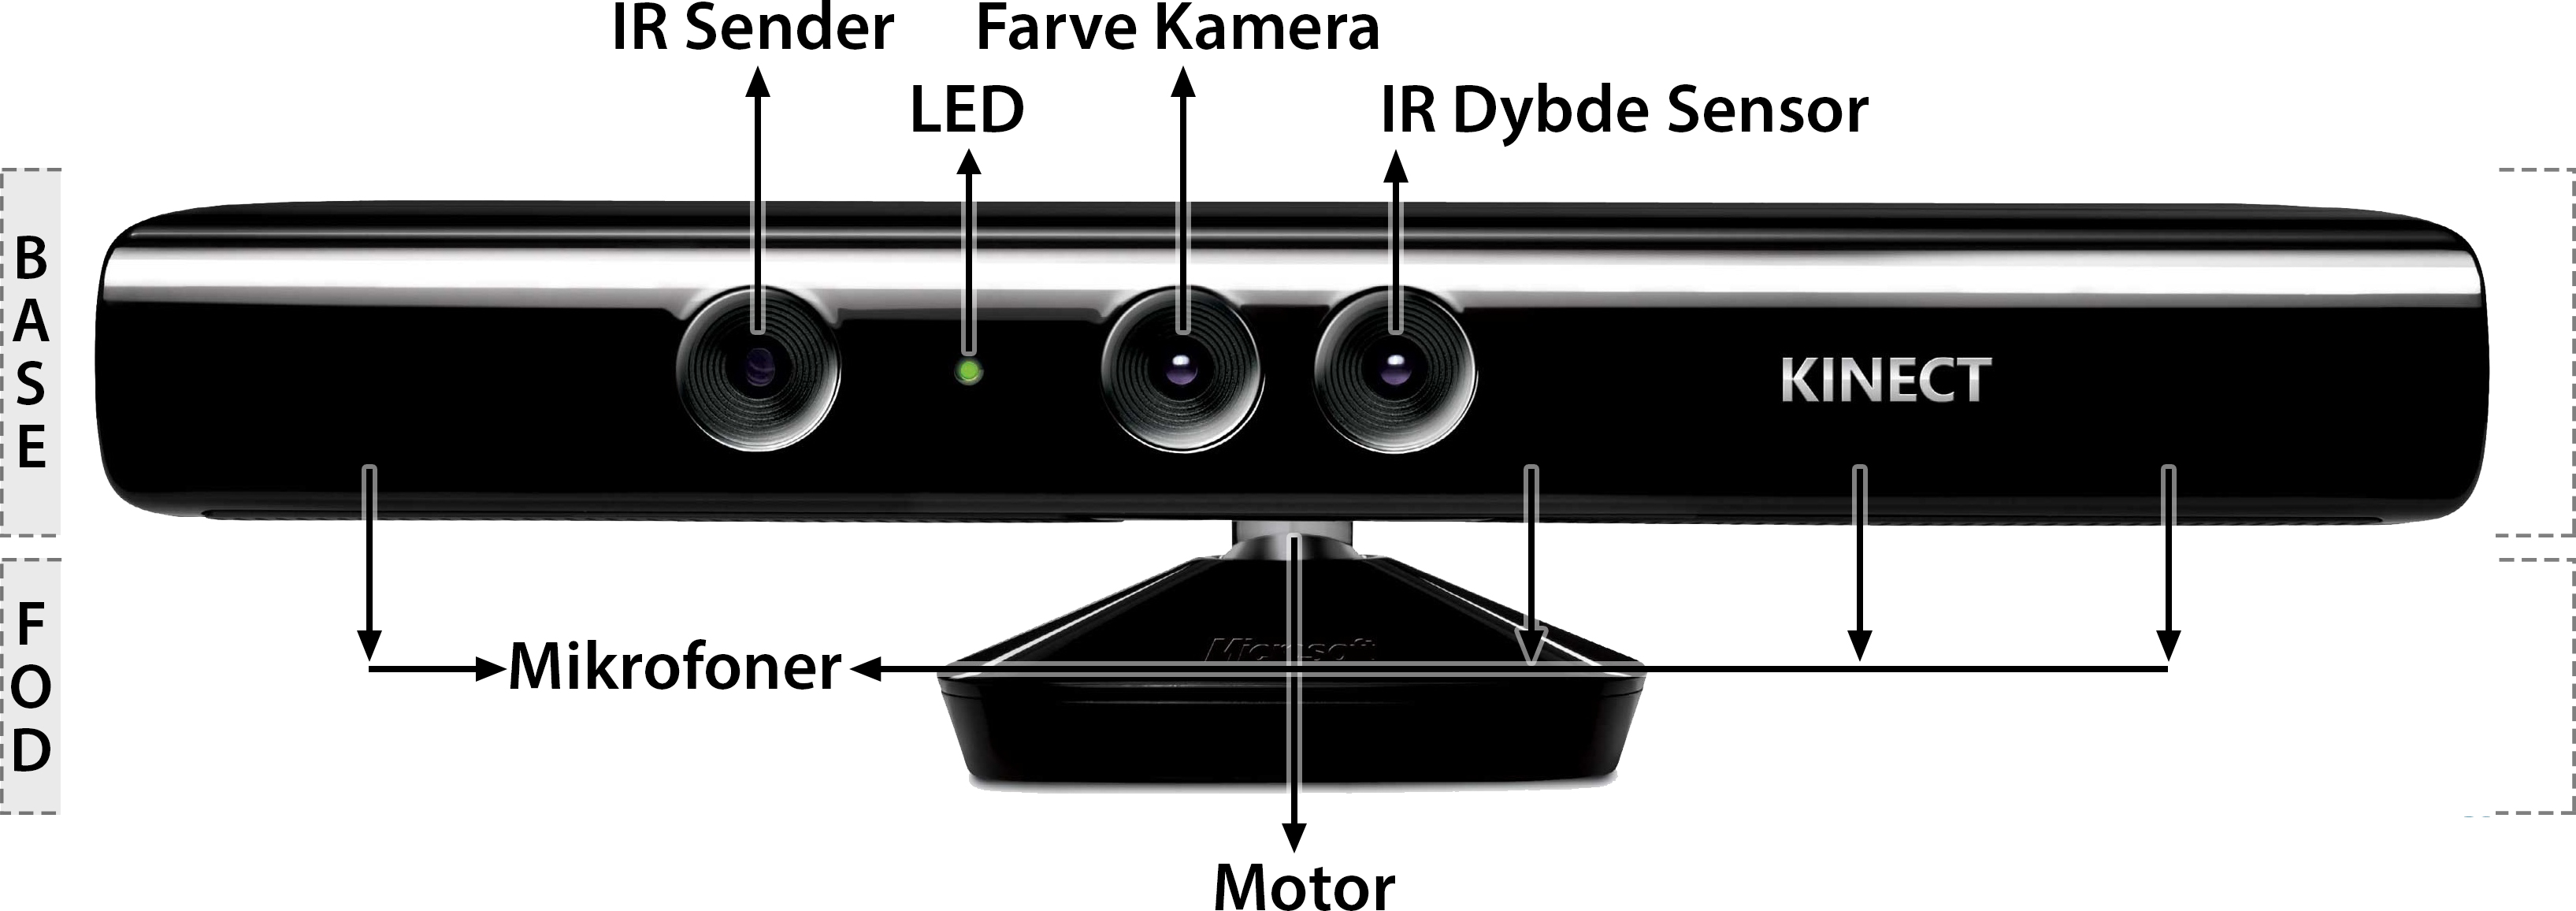
\includegraphics[width=1.0\textwidth]{kinect}
\caption{Microsoft Kinect for Windows}
\label{kinect:opbygning}
\end{figure}

\subsubsection{Prime Sense PS1080}
\thilemann{Skriv noget om at det er den chip der står for genkendelse af bevægelser osv. Se evt. \url{http://www.primesense.com/solutions/technology/}.}

\subsubsection{Farvekamera}
For at gøre Kinecten i stand til at se, er den udstyret med et farvekamera som er placeret ca. i midten.
Et farvekamera kan være nyttigt i spil, hvor man ønsker at vise spilleren fysik på skærmen eller hvis man benytter sin Kinect til gruppechat (som et webcam).
Videoen bliver sendt som en RGB videostrøm med mulighed for en opløsning på 1280x960 med en opdateringshastighed på 12 billeder i sekundet eller en lavere opløsning på 640x480 og 30 billeder i sekundet, hvis man ønsker en mere ”flydende” videostrøm~\cite{kinectForWindowsFeatures}.
Det har en horisontal betragtningsvinkel på 57\degree~og en vertikal betragtningsvinkel på 43\degree, hvilket kan være interessant ift. det miljø hvori Kinecten skal bruges.

\subsubsection{Infrarød (IR) sender}
Metoden Kinecten benytter for at bestemme personers placeringer deres afstand fra Kinecten er vha. den infrarøde (IR) sender, som udsender et infrarødt lys der reflekteres så snart de rammer et objekt i rummet. 
Disse signaler bliver fanget af en anden sensor på Kinecten; nemlig den infrarøde dybde sensor.

\subsubsection{IR dybde sensor}
Når det infrarøde lys bliver reflekteret tilbage mod Kinecten, bliver det opfanget af dybde sensoren, som konverterer lyset til dybde information, hvori man har en per-pixel afstand til de objekter der er tilstede i billedet.

\subsubsection{Mikrofoner}
Kinecten er også i stand til at optage lyd via de indbyggede mikrofoner.
Dette er dog ikke det eneste mikrofonerne kan benyttes til; de kan også benyttes som en alternativ metode (til dybde billeder) til at bestemme afstand og retning fra f.eks. en person der taler.
Rækken af mikrofoner består af 4 stk. som er placeret på fronten af Kinecten.
En enkelt mikrofon sidder i venstre side mens de tre andre er placeret til højre, hvilket gør det muligt at triangulere lydsignaler for at bestemme retningen af lydkilden.
Flere mikrofoner gør det også muligt at lave "noise-suppression" ift. omgivelserne, hvis man benytter Kinect, mens man spiller, til at kommunikerer med sine med-/modspillere således at unødig støj filtreres fra~\cite[s.~15]{kinectProgrammingGuide}.

\subsubsection{Motor til justering af vinklen}
For at gøre det muligt for en Kinect at operere i flere forskellige miljøer og placeringer, er der indbygget en lille motor til at justere vinklen mellem Kinecten og foden den står på.
Den kan bevæge sig fra 0\degree~til 27\degree~ (op) og fra 0\degree~til -27\degree~(ned).
Denne funktionalitet er ideel hvis man ønsker at kalibrere Kinecten ift. dens fysiske placering og de omgivelser man ønsker at bruge den i.
Dog anbefaler Microsoft at man ikke benytter motoren kontinuert i sine programmer, da den ikke tåler vedvarende belastninger~\cite{kinectDocElevationAngle}.

\subsubsection{LED}
Mellem kameraet og IR senderen er der placeret en status LED, der fortæller om driverne til Kinecten er indlæst korrekt eller ej.
Dette kan være nyttigt for udviklere, da det giver sikkerhed for at kommunikationen mellem PC og Kinect er ok~\cite[s.~15]{kinectProgrammingGuide}.

\subsubsection{Accelerometer}
Kinect er også udstyret med et 3-akse accelerometer, som udvider den til andre anvendelsesområder end blot at følge (tracke) objekter og kropsbevægelser.
Det er konfigureret til at give målinger fra -2g til 2g (bedre til langsomme bevægelser ifht. højere værdier)~\cite{kinectAccelerometer}.
Målingerne  er opbygget som en 3D vektor som peger mod tyngdekraften (gulv-planet), hvilket f.eks. gør det muligt at detektere om den er monteret korrekt (ovenpå eller under et fladskærms tv), således dens tilt kan korrigeres vha. den indbyggede motor.
En anden interessant anvendelsesmulighed er at accelerometeret kan benyttes til at give bedre 3D projektioner i Augmented Reality.
Ifølge dokumentationen~\cite{kinectDocAccelerometer}, er det præcist ned til en grad, dog med en nøjagtighed der kan varierer med op til 3 grader i forhold til rumtemperaturen.
De skriver endvidere i dokumentationen at der kan kompensateres for denne unøjagtighed ved at sammenligne den vertikale måling (y-aksen i accelerometerets koordinatsystem) med den benyttede gulvplans dybdedata.


\section{Kinect for Windows SDK}
Da Kinecten udkom fandtes der intet officielt Software Development Kit (SDK) som udviklere kunne bruge til at lave deres egne applikationer, men derimod kun SDK'er udviklet af tredjepartsudviklere som libfreenect\footnote{Udviklet af OpenKinect (\url{http://www.openkinect.org})} og OpenNI\footnote{Open Natural Interaction (\url{http://www.openni.org})}, som er et SDK for 3D sensorer, der kan benyttes med PrimeSense's sensor driver kaldet SensorKinect\footnote{\url{https://github.com/avin2/SensorKinect}}, hvis man ønsker at benytte OpenNI sammen med Kinect.

\thilemann{måske beskrivelse af windows SDK vs.Libfreekinect og openni?}

Anerledes er det i dag, hvor der findes et officielt SDK i version 1.8\footnote{Udgivet 17 september, 2013~\cite{kinectSDK18}}, som åbner op for al funktionalitet i Kinecten med support fra Microsoft.

API'en er bygget op omkring en solid forståelse for menneskers bevægelser og karaktertræk således API'en kan fungere som et interface der kan genkende skeletelle bevægelser, følge ansigter, genkende gestus og tale.
Med Microsoft Kinect Toolkit installeret kan man endvidere få adgang til Microsoft.Kinect.Toolkit namespacet, hvilket indeholder Kinect Fusion der gør det muligt at rekonstruere 3D objekter ud fra Kinectens kamera og dybdebilleder fra IR sensorene.~\cite{kinectForWindowsFeatures}


\subsection{Kinect API}\label{kinect:kinectapi}
For at benytte Kinect API er det første skridt at tilføje en reference til biblioteket i projektet i Visual Studio, og dernæst at tilføje namespacet via \lstinline!using Microsoft.Kinect;!.
Herefter skal Kinecten initialiseres for at få adgang til dens forskellige sensorer. Som det ses af \cref{kinect:apiopbygning}, er API'en inddelt i klasser alt efter hvilken sensor man vil have adgang til, og hvad funktionen af den pågældende sensor er.
Dette faktum ligger også til grund for de følgende eksempler på brug af Kinectens sensorer.

\begin{figure}
\centering
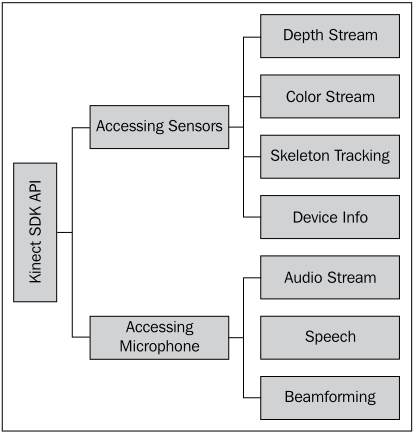
\includegraphics[width=0.6\textwidth]{kinect_api_opbygning}
\caption{Kinect API opbygning \thilemann{Tikz-ify this...}}
\label{kinect:apiopbygning}
\end{figure}


\subsubsection{Opret forbindelse til Kinect}

\subsubsection{Video}

\begin{lstlisting}[style=csharp,caption={Kinect SDK kamera},label=kinect:sdk-kamera]

\end{lstlisting}

\subsubsection{Dybdebillede}


\subsection{Coding4Fun Kinect Toolkit}
Coding4Fun Kinect Toolkit giver adgang til en række extension metoder som fungerer som et lag der binder sig til Kinect API'en ved at abstrahere de mere lav-niveau detaljer væk. Det betyder bl.a. at man slipper for at konvertere videostrømmen fra kameraet om til en \lstinline!Image! type som nemt kan benyttes sammen med de indbyggede .NET klasser.

Resten af denne sektion giver eksempler på brug vha. Coding4Fun Kinect Toolkit, der modsvarer eksemplerne fra \cref{kinect:kinectapi}, hvor Kinect API'en er beskrevet.

\subsubsection{Opret forbindelse til Kinect}

\subsubsection{Kamera}

\subsubsection{Dybdebillede}